

\tikzset{every picture/.style={line width=0.75pt}} %set default line width to 0.75pt        

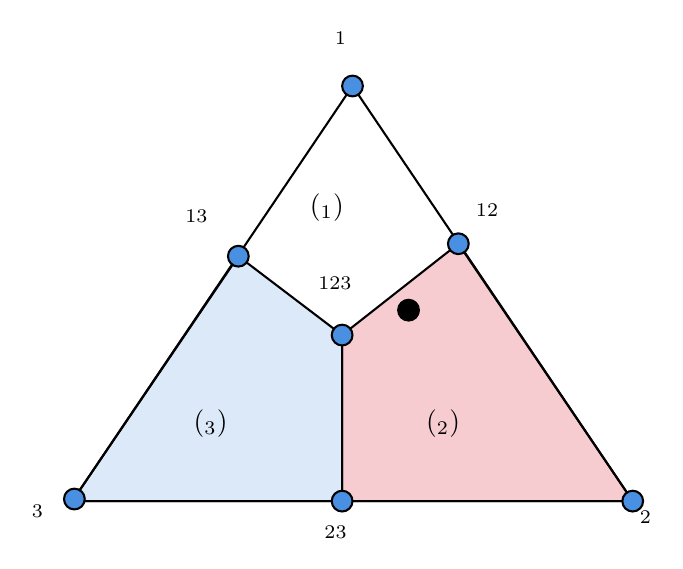
\begin{tikzpicture}[x=0.75pt,y=0.75pt,yscale=-1,xscale=1]
%uncomment if require: \path (0,300); %set diagram left start at 0, and has height of 300

%Shape: Polygon [id:ds12997950611396247] 
\draw  [fill={rgb, 255:red, 74; green, 144; blue, 226 }  ,fill opacity=0.2 ] (230,250) -- (230,170) -- (180,132) -- (100,250) -- cycle ;
%Shape: Triangle [id:dp2663618049578823] 
\draw   (235,50) -- (370,250) -- (100,250) -- cycle ;
%Shape: Polygon [id:ds41194641592346326] 
\draw  [fill={rgb, 255:red, 208; green, 2; blue, 27 }  ,fill opacity=0.2 ] (286,126) -- (370,250) -- (230,250) -- (230,170) -- cycle ;
%Shape: Circle [id:dp6296340315249684] 
\draw  [fill={rgb, 255:red, 0; green, 0; blue, 0 }  ,fill opacity=1 ] (257,158) .. controls (257,155.24) and (259.24,153) .. (262,153) .. controls (264.76,153) and (267,155.24) .. (267,158) .. controls (267,160.76) and (264.76,163) .. (262,163) .. controls (259.24,163) and (257,160.76) .. (257,158) -- cycle ;
%Shape: Circle [id:dp5483903323436823] 
\draw  [fill={rgb, 255:red, 74; green, 144; blue, 226 }  ,fill opacity=1 ] (281,126) .. controls (281,123.24) and (283.24,121) .. (286,121) .. controls (288.76,121) and (291,123.24) .. (291,126) .. controls (291,128.76) and (288.76,131) .. (286,131) .. controls (283.24,131) and (281,128.76) .. (281,126) -- cycle ;
%Shape: Circle [id:dp8527922823860563] 
\draw  [fill={rgb, 255:red, 74; green, 144; blue, 226 }  ,fill opacity=1 ] (175,132) .. controls (175,129.24) and (177.24,127) .. (180,127) .. controls (182.76,127) and (185,129.24) .. (185,132) .. controls (185,134.76) and (182.76,137) .. (180,137) .. controls (177.24,137) and (175,134.76) .. (175,132) -- cycle ;
%Shape: Circle [id:dp7738782974933459] 
\draw  [fill={rgb, 255:red, 74; green, 144; blue, 226 }  ,fill opacity=1 ] (230,50) .. controls (230,47.24) and (232.24,45) .. (235,45) .. controls (237.76,45) and (240,47.24) .. (240,50) .. controls (240,52.76) and (237.76,55) .. (235,55) .. controls (232.24,55) and (230,52.76) .. (230,50) -- cycle ;
%Shape: Circle [id:dp23232151108326793] 
\draw  [fill={rgb, 255:red, 74; green, 144; blue, 226 }  ,fill opacity=1 ] (365,250) .. controls (365,247.24) and (367.24,245) .. (370,245) .. controls (372.76,245) and (375,247.24) .. (375,250) .. controls (375,252.76) and (372.76,255) .. (370,255) .. controls (367.24,255) and (365,252.76) .. (365,250) -- cycle ;
%Shape: Circle [id:dp16405524479010358] 
\draw  [fill={rgb, 255:red, 74; green, 144; blue, 226 }  ,fill opacity=1 ] (225,250) .. controls (225,247.24) and (227.24,245) .. (230,245) .. controls (232.76,245) and (235,247.24) .. (235,250) .. controls (235,252.76) and (232.76,255) .. (230,255) .. controls (227.24,255) and (225,252.76) .. (225,250) -- cycle ;
%Shape: Circle [id:dp40899181563799814] 
\draw  [fill={rgb, 255:red, 74; green, 144; blue, 226 }  ,fill opacity=1 ] (96,249) .. controls (96,246.24) and (98.24,244) .. (101,244) .. controls (103.76,244) and (106,246.24) .. (106,249) .. controls (106,251.76) and (103.76,254) .. (101,254) .. controls (98.24,254) and (96,251.76) .. (96,249) -- cycle ;
%Shape: Circle [id:dp7696235932553328] 
\draw  [fill={rgb, 255:red, 74; green, 144; blue, 226 }  ,fill opacity=1 ] (225,170) .. controls (225,167.24) and (227.24,165) .. (230,165) .. controls (232.76,165) and (235,167.24) .. (235,170) .. controls (235,172.76) and (232.76,175) .. (230,175) .. controls (227.24,175) and (225,172.76) .. (225,170) -- cycle ;

% Text Node
\draw (264,156.4) node [anchor=north west][inner sep=0.75pt]    {$\prior$};
% Text Node
\draw (225,22.4) node [anchor=north west][inner sep=0.75pt]    {$\belief _{1}$};
% Text Node
\draw (372,253.4) node [anchor=north west][inner sep=0.75pt]    {$\belief _{2}$};
% Text Node
\draw (79,250.4) node [anchor=north west][inner sep=0.75pt]    {$\belief _{3}$};
% Text Node
\draw (157,204.4) node [anchor=north west][inner sep=0.75pt]    {$\opt( \aaction_{3})$};
% Text Node
\draw (269,204.4) node [anchor=north west][inner sep=0.75pt]    {$\opt( \aaction_{2})$};
% Text Node
\draw (213,100.4) node [anchor=north west][inner sep=0.75pt]    {$\opt( \aaction_{1})$};
% Text Node
\draw (293,105.4) node [anchor=north west][inner sep=0.75pt]    {$\belief _{12}$};
% Text Node
\draw (217,140.4) node [anchor=north west][inner sep=0.75pt]    {$\belief _{123}$};
% Text Node
\draw (220,260.4) node [anchor=north west][inner sep=0.75pt]    {$\belief _{23}$};
% Text Node
\draw (153,108.4) node [anchor=north west][inner sep=0.75pt]    {$\belief _{13}$};


\end{tikzpicture}